\cleardoublepage

\chapter{Casos de Estudio}
\label{ch:Capitulo5}

\section{Potencial como prototipo para evaluación de solución domótica}
La modularidad y movilidad de esta suite domótica permite realizar despliegues rápidos ante un gran abanico de necesidades. Partiendo de un kit básico, compuesto por el nodo principal, unas cuantas placas genéricas equipadas con un modulo esp8266 y unos cuantos sensores y actuadores, se puede prototipar una solución de domótica automática personalizada para un situación, evaluar su utilidad y planificar una instalación mas profesional si las pruebas obtienen resultados deseados.


\section{Aplicando la solución en un entorno propuesto}
\label{ch:Capitulo5.1}
El escenario se desarrolla en una bodega de uso domestico situado bajo tierra. El acceso a la misma se encuentra dentro de un hogar a través de unas escaleras que bajan hasta la estancia donde una pareja de toneles fermentan vino de cosecha propia de la unidad familiar que reside en la casa. Originalmente este espacio había sido diseñado como almacén y no dispone de medios electrónicos salvo el cableado de iluminación que dispone de un interruptor en la parte superior de las escaleras y una toma de enchufe al final de las mismas.

Existe una serie de condiciones previstas para una buena conservación del vino embotellado en una bodega , humedad relativa de tu bodega debe estar entre el 65 por ciento y el 75 por ciento. En una bodega demasiado seca pueden llegar a resecarse los tapones, mientras que una excesivamente húmeda presenta el peligro de que se alteren los tapones y las etiquetas debido a la aparición de mohos. La temperatura debe oscilar entre los 10-15C y debe ser, en lo posible, constante. Por otra parte, debe estar bien ventilada pero sin grandes corrientes de aire. Una bodega demasiado fresca ralentiza la evolución del vino y puede ser la causa de que se produzca la precipitación de cristales de tartratos. Por el contrario, en una bodega en la que la temperatura es demasiado alta, el vino tiende a evolucionar más rápidamente y esto puede llegar a traducirse en un envejecimiento prematuro


Como estrategia, un sensor tomara medidas indefinidamente y los volcara en un fichero/BBDD para recortar los tiempo de respuesta, evitando así esperar a que el sensor haga la toma de medidas en el momento de la solicitud y obteniéndolas en su lugar del último registro que tengamos. Un último problema con el que hay que lidiar es su baja precisión limitada a enteros, por lo que no podemos esperar obtener un dato preciso a la décima de la temperatura y humedad. Esto sin embargo no es un problema real dada la naturaleza del proyecto, ya que no necesitamos un grado de precisión menor a la unidad para tomar acciones o informar al usuario.

\section{Caso de uso: Vincular un dispositivo registrado a una habitación}
\label{ch:Capitulo5.2}
El usuario previamente ha registrado en la aplicación una habitación para esta bodega y ha registrado una luz de tipo led. En este momento desea poder vincular esa luz a la bodega, de forma que pueda encenderla y apagarla y observar el estado actual de la luz desde su aplicación. A continuación se describe el proceso por el cual el usuario selecciona las características de la vinculación que va a llevar a cabo (eligiendo la luz, la habitación a la cual vincularla, el modelo de la placa en la cual montará la luz y el pin en el que la conectará) y conecta la placa por USB a la Raspberry (para que el servidor genere, compile y cargue los scripts necesarios en la placa para que ésta interactúe con la luz y con el nodo principal). Cuando este proceso finaliza, la placa está correctamente vinculada y tanto el backend como el frontend están alineados en información, de forma que el backend será capaz de comunicarse directamente con la luz y retransmitir su estado al frontend, y el frontend podrá controlar su estado mediante comandos lanzados al backend. El usuario podrá observar que la luz ya aparece vinculada estrictamente a la bodega.
El diagrama explicativo de este caso de uso es la Figura \ref{fig:usecase1}

\begin{figure}[hbt!]
\centering
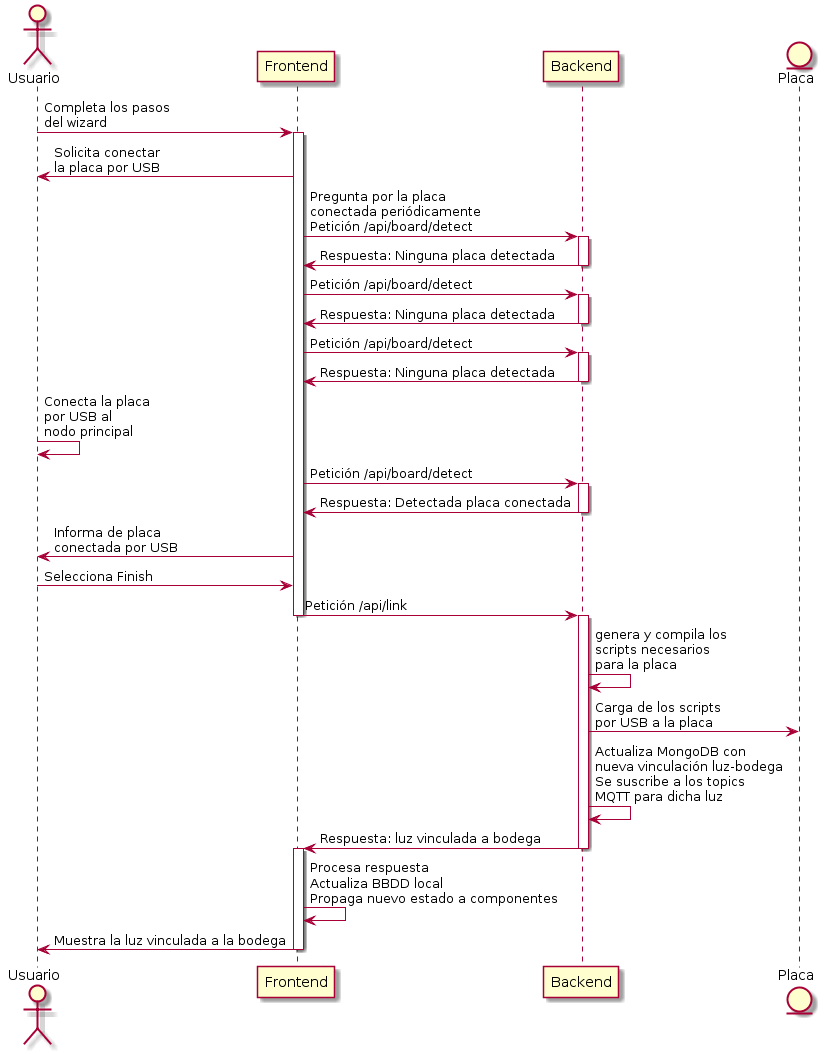
\includegraphics[height=8in]{figures/diagrams/use-cases/linkRoom.png}
\caption[usecase1]{Diagrama de comunicación entre frontend, backend y placa para vincular un dispositivo a una habitación\footnotemark}
\label{fig:usecase1}
\end{figure}

\subsection{Fase 1: Lado aplicación móvil}
\label{ch:Capitulo5.2.1}
\begin{enumerate}
\item  El usuario accede al menú en la pestaña inferior derecha, a su vez al menú \textit{Connect}, localiza la thing que quiere vincular (representada mediante el \verb|thing-block.component|, en este caso la luz de tipo led y procede a deslizarla hacia la izquierda y pulsar en el botón \textit{Link}. Esto desencadena el envío de un evento que escucha el componente padre, \verb|connect.ts|, y lo vincula a la ejecución de su método \verb|linkThing|. Éste se encarga de mostrar el elemento modal que contendrá el asistente de vinculación de la thing a una habitación, cuya lógica estará dispuesta en \verb|wizard-link.modal|. A partir de aquí a cada paso del asistente se le requerirá al usuario información imprescindible para la vinculación, y no podrá avanzar al siguiente paso con el botón \textit{Next} hasta que cumpla lo solicitado en cada paso.

\item  En un primer paso, se mostrará al usuario la lista de habitaciones reconocibles mediante su nombre personalizado, para que elija la habitación a la cual quiere vincular esta luz, en este caso, la bodega. Una vez elegido, este dato se preserva hasta el final del asistente.

\item En el segundo paso, se mostrará al usuario la lista de placas disponibles compatibles, con el fin de que elija el modelo de placa sobre el cual montará la luz. En el siguiente paso, se pide al usuario el pin sobre el cual montará la luz. Ambos datos se preservan hasta el final del asistente.

\item  En el último paso, se muestra al usuario un breve mensaje descriptivo de la acción que va a llevarse a cabo con sus elecciones, y se le insta a conectar la placa en la cual ha montado la luz al puerto USB de la Raspberry Pi. Sólo cuando esto ocurra, explicado en más detalle en la Fase Auxiliar de este caso de uso, se permitirá al usuario que lance el proceso de vinculación con el botón \textit{Finish}, el cual ejecuta el método \verb|closeAndFinish|, que a su vez delega el proceso de vinculación en el método \verb|linkRoom| de la \verb|thing.store.ts|, pasando como parámetros la thing vinculada, el id de la habitación, el modelo de placa y el pin asignado.

\item  Este método \verb|linkRoom| llamará a su vez (con el id de thing, el modelo de thing, el id de habitación, el modelo de placa y el pin) al método \verb|linkRoom| del \verb|linkProvider| (\verb|api-link.service.ts|), el cual se encarga de comunicar con la api que atiende el servidor en el endpoint \verb|/api/link|. A través del método privado \verb|create|, lanza una petición http de tipo POST, extendida al endpoint \verb|/api/link|, con payload todos los parámetros descritos.
\end{enumerate}

Estos pasos son encadenados mediante promesas (Objetos \textbf{Promise} del ECMASCRIPT 6), y tras la respuesta del servidor en la fase 2 de este caso de uso, las promesas se desenrollarán progresivamente hacia atrás en la fase 5, cubriendo los flujos de resolución (si la respuesta es positiva) o los flujos de rechazo (si la respuesta es negativa), detallados en la fase 3.

\subsection{Fase 2: Lado servidor}
\label{ch:Capitulo5.2.2}
\begin{enumerate}
\item  El router del servidor en \verb|router.js| detecta el endpoint \verb|/api/link| y redirige la petición hacia el \verb|link.router.js|, el cual detecta a su vez la ruta \verb|/| y el tipo POST y redirige la petición a ser controlada por el método \verb|linkRoom| del \verb|link.controller.js|. Obtiene del body de la petición todos los parámetros detallados en el paso 5 de la fase anterior.

\item  El método \verb|linkRoom| llamará al método \verb|compileAndUploadToBoard| del \verb|shell.service.js|, que ejecuta el script de shell \verb|sketchgenerator| para una especificación dada, el cual se encarga de obtener el código necesario, compilarlo y cargarlo en la placa conectada por USB a la Raspberry Pi.

\item  Si la ejecución del script finaliza con éxito, actualizará la thing en la MongoDB con la nueva habitación vinculada, en el campo \verb|linkedRoomId|, con el método \verb|findOneAndUpdate| del modelo \textbf{Thing} (esquema de la DB).

\item  Si se actualiza con éxito, entonces llamará al método \verb|generateSubscriptionData| del \verb|thingHelper| (\verb|thing.helper.js|) el cual, a partir del tipo de la thing, obtiene una instancia con la funcionalidad específica necesaria para procesar tanto el status como las respuestas recibidas por \gls{mqtt}.

\item  Con esta información, llamará al \verb|addSubscription| del \verb|mqtt.service.js|, el cual suscribirá al topic \textit{idThing/answer} y a \textit{idThing/status} y guarda en una lista interna de suscripciones las 2 nuevas suscripciones, donde asocia futuros mensajes en dichos topics a los métodos \verb|processAnswer| y \verb|processStatus| respectivamente.

\item  Posteriormente, actualizará la habitación en la MongoDB con la nueva thing vinculada, con el método \verb|update| del modelo \textbf{Room} (esquema de la DB).

\item  Si se actualiza con éxito, desencadena la resolución con éxito de la petición http, enviando de vuelta una respuesta con código http 200 acompañado de un body que contiene un sencillo mensaje descriptivo de éxito.

\item  Si alguno de los pasos falla, desencadena la resolución con fracaso de la petición http, enviando de vuelta una respuesta con código http 500 acompañado de un body que contiene un sencillo mensaje descriptivo del error ocurrido.
\end{enumerate}

\subsection{Fase 3: Lado aplicación móvil}
\label{ch:Capitulo5.2.3}
\begin{enumerate}
\item  La última promesa que aguarda al final de la fase 1 de este caso de uso, tras recibir respuesta exitosa por parte del servidor sobre la petición que realizó (recibe un código 200, y si fuera un 400/500, se procedería a controlar el error con el método heredado \verb|handleError| e iniciar la ejecución del flujo de rechazo), resuelve la promesa, devuelta al flujo a la espera en \verb|linkRoom| de la \verb|thing.store.ts|.

\item  El flujo de éxito actualizará el campo \verb|linkedRoomId| de la thing, añadiendo el id de la habitación recién vinculada, y tras esto, se utiliza el método \verb|set| del \verb|ThingDatabaseService| (\verb|thing.service.db.ts|), que se encarga de actualizar la DB local del dispositivo. De la misma forma, tras esto, se acude al método \verb|linkThingToRoom| de la \verb|room.store.ts|, que se encargará en paralelo de igualmente actualizar la habitación correspondiente con la nueva lista de things vinculadas a ella, y actualizar con el método \verb|set| del \verb|RoomDataBaseService| (\verb|room.service.db.ts|) que se encarga de actualizar la DB local del dispositivo.

\item  Una vez actualizada la DB local de la aplicación móvil, se llama al método privado \verb|refreshList| de la clase actual, \verb|ThingStore|, con el objetivo de cargar la reciente lista actualizada en la DB y propagar el nuevo valor de esta lista (con sus elementos recién actualizados) a todos aquellos interesados en la aplicación. Esto se consigue mediante la actualización del elemento \textbf{Observable} \verb|_currentThingsObservable|, que mediante el patrón de Observer/Subscribe, informa a todos los suscriptores interesados en los cambios de dicho campo (gracias a esto, la lista inicial de things en el menú \textit{Connect} será actualizada con la reciente vinculación de la thing a su habitación). Este mismo proceso ocurre también en paralelo en \verb|RoomStore| pero aplicado a la lista de habitaciones. Por último, se resuelve la promesa, devuelta en este método \verb|linkRoom| al método \verb|closeAndFinish| del \verb|wizard-modal.ts|. 

\item  Una vez se ejecuta el flujo de éxito en el componente \verb|wizard-link.modal|, se muestra un breve mensaje de tipo toast informando del éxito en la vinculación mediante el uso del método \verb|showToast| del servicio \verb|toast.service.ts|.
\end{enumerate}

\subsection{Fase Auxiliar: detección del dispositivo conectado por USB}
\label{ch:Capitulo5.2.4}
Precondiciones:
    -Al iniciar la aplicación servidor, ha sido inicializado el servicio de detección de dispositivos conectados por USB, \verb|usb.service.js| mediante el método \verb|initListening| de este mismo. Así, cada conexión, desconexión o cambio de dispositivo conectado por los puertos USB de la Raspberry Pi será monitorizado.

\begin{enumerate}
\item  Cuando el usuario alcanza el último paso del asistente de vinculación de dispositivos a habitaciones del \verb|wizard-link.modal.ts|, se lanza el método \verb|startPollingUsbBoard| de la \verb|board.store.ts|, el cual se encarga de lanzar periódicamente el método interno \verb|_retrieveDetectedUsbBoard|, a intervalos de 2 segundos, y se suscribe a los cambios del \textbf{Observable} retornado por \verb|detectedBoardObserver| de la \verb|board.store.ts|. 

\item  El método \verb|startPollingUsbBoard| se encarga de llamar al método \verb|getUsbConnectedBoard| de la \verb|boardProvider| (\verb|api-board.service.ts|), el cual se encarga de comunicar con la api que atiende el servidor en el endpoint \verb|/api/board|. A través del método privado \verb|create|, lanza una petición http de tipo GET, extendida al endpoint \verb|/api/board/detect|. 

\item  El router del servidor en \verb|router.js| detecta el endpoint \verb|/api/board| y redirige la petición hacia el \verb|board.router.js|, el cual detecta a su vez la ruta \verb|/detect| y el tipo GET y redirige la petición a ser controlada por el método \verb|getUSBConnectedBoard| del \verb|board.controller.js|.

\item  Este método solicita al \verb|usb.service.js| si existe una placa conectada en ese mismo momento mediante el método \verb|getCurrentConnectedUSB|. Si el servicio había registrado un dispositivo conectado, lo retornará, desencadenando la resolución con éxito de la petición http, enviando de vuelta una respuesta con código http 200 acompañado de un body que un objeto \textbf{Board} (según esquema de la MongoDB) con la información de la placa. Si no había ningún dispositivo registrado, desencadenará la resolución de fallo de la petición http, enviando de vuelta una respuesta con código http 500 acompañado de un breve mensaje descriptivo de la ausencia de dispositivos conectados por USB.

\item  Tras recibir respuesta exitosa por parte del servidor sobre la petición que realizó (recibe un código 200, y si fuera un 400/500, se procedería a controlar el error con el método heredado \verb|handleError| e iniciar la ejecución del flujo de rechazo), resuelve la promesa del paso 2, recuperando el flujo a la espera en \verb|getUsbConnectedBoard| de la \verb|board.store.ts|.

\item  Éste, dependiendo de la respuesta, actualizará el valor \verb|_detectedUsbBoard| existente (si es positiva, añadirá un objeto con la información disponible de dicha board; si la respuesta es negativa, añadirá un objeto vacío). Mediante el patrón Observer/Subscribe, avisará al suscriptor del \verb|wizard-link.modal.ts|, para que, al detectar cuando existe una board conectada por USB, habilita el botón \textit{Finish}.
\end{enumerate}

\section{Caso de uso: Encender un dispositivo luminoso de tipo led}
\label{ch:Capitulo5.3}
El usuario ha registrado en la aplicación una habitación para esta bodega, ha registrado una luz de tipo led y la ha vinculado a dicha bodega mediante lo explicado en el caso de uso anterior. En este momento, el usuario decide encender dicha luz. El proceso descrito a continuación detalla cómo el frontend responde al input del usuario que desplaza el interruptor de luz en el componente visual, comunicando el comando de encendido al servidor mediante una petición http, cómo el backend procesa el comando para entender qué acción debe llevar a cabo y envía por MQTT el mensaje adecuado a la luz adecuada, y cómo se produce la respuesta desde la placa, el backend reacciona a la respuesta por MQTT de la placa, actualiza el estado de la luz en su base de datos y devuelve la petición http al frontend, el cual procesa la respuesta desplazando el botón e iluminando el componente visual de la luz.
El diagrama explicativo de este caso de uso se muestra en la Figura \ref{usecase2}.

\begin{figure}[hbt!]
\label{usecase2}
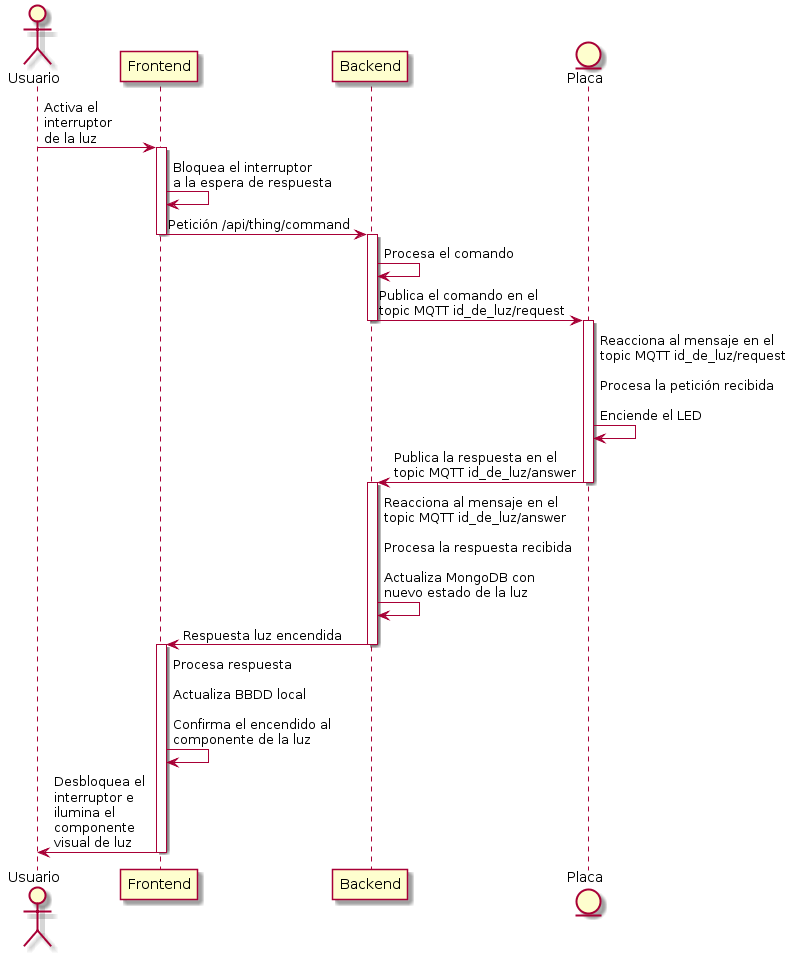
\includegraphics[height=8in]{figures/diagrams/use-cases/turnOnLight.png}
\caption[usecase2]{Diagrama de comunicación entre frontend, backend y placa para encender un dispositivo led\footnotemark}
\end{figure}

\subsection{Fase 1: Lado aplicación móvil}
\label{ch:Capitulo5.3.1}
\begin{enumerate}
 \item  Desde uno de los componentes visuales, bien sea el \verb|room-preview.component.ts|, o sea el \verb|light-component.ts|, tras interacción del usuario con el toggle (interruptor) de esta luz, se desencadena el método \verb|toggleMainLight| o \verb|toggleLight| respectivamente, los cuáles ejecutan un algoritmo similar que por un lado deshabilita el interruptor para el usuario durante el breve lapso de procesamiento que ocurre hasta que se reciba una respuesta en la fase 5 de este caso de uso, y por otro lado llama al método \verb|turnOn| de la \verb|thing.store.ts| con la información de la thing en cuestión (nuestra luz) como parámetro.
 
 \item  Éste llamará al método privado \verb|setProperty| pasándole la thing y un objeto de la clase \textbf{CommandRequestModel} con parámetros de comando para encender.
 
 \item  \verb|setProperty| delega en el método \verb|setProperty| del \verb|thingProvider| (\verb|api-thing.service.ts|), el servicio que se encarga de comunicar con la api que atiende el servidor en el endpoint \verb|/api/thing|. A través del método privado \verb|update|, lanza una petición http de tipo PUT, extendida al endpoint \verb|/api/thing/command/:id|, con el id de la thing como parámetro id de la url, y el comando como payload.
 
 Estos pasos son encadenados mediante promesas (Objetos \textbf{Promise} del ECMASCRIPT 6), y tras la respuesta del servidor en la fase 4 de este caso de uso, las promesas se desenrollarán progresivamente hacia atrás en la fase 5, cubriendo los flujos de resolución (si la respuesta es positiva) o los flujos de rechazo (si la respuesta es negativa).
 \end{enumerate}

\subsection{Fase 2: Lado servidor}
\label{ch:Capitulo5.3.2}
\begin{enumerate}
\item  El router del servidor en \verb|router.js| detecta el endpoint \verb|/api/thing| y redirige la petición hacia el \verb|thing.router.js|, el cual detecta a su vez la ruta \verb|/command/:id| y el tipo PUT y redirige la petición a ser controlada por el método \verb|processCommand| del \verb|thing.controller.js|. Obtiene del body de la petición el comando solicitado.

\item  Éste realiza una acceso a la MongoDB mediante el método \verb|findOne| del modelo \textbf{Thing} (esquema de la DB), para obtener los datos almacenados de la thing en cuestión mediante el id extraído de la url.

\item  Si existe y logra los datos, llamará al método \verb|getThingControllerInstance| del \verb|thingHelper| el cual, a partir del tipo de la thing (tipo light), obtiene una instancia con la funcionalidad específica necesaria para procesar un comando y enviarlo al dispositivo. En este caso, el método será el \verb|processRequest| del \verb|light.controller.js|.

\item  En el \verb|light.controller.js|, se utiliza el método interno \verb|_arePropertiesAlreadyLoaded| para comprobar, a partir del comando y los datos almacenados de la thing, si los cambios de propiedades que indica el comando implican un cambio real en el estado actual (almacenado) del dispositivo. Esto se hace para evitar comandos en paralelo que puedan dar lugar a comportamientos inesperados.

\item  Si el comando debe efectivamente enviarse, se procede a extraer el string equivalente del comando, y registrar una nueva entrada en la lista interna de comandos pendientes mediante el método interno \verb|_cacheRequestFlow|. Este sistema permite guardar la traza de un comando dirigido hacia una thing en particular con unas propiedades en particular con el objetivo de asociar a dicha traza un flujo de éxito y otro de fracaso, que se ejecutarán respectivamente cuando en la fase 4 de este caso de uso se recoja la respuesta de éxito o fracaso del comando en el dispositivo.

\item  Se llama entonces al método \verb|publish| del \verb|mqtt.service.js|, que se encargará a su vez de publicar el mensaje final en el topic compuesto \textit{thingId/request}.
\end{enumerate}

\subsection{Fase 3: Lado dispositivo}
\label{ch:Capitulo5.3.3}
\begin{enumerate}
\item La placa se encuentra en un estado de continua escucha del topic \verb|request| para su propio identificador. El proceso de resolución de mensajes entrantes por parte del servidor, recibe un string con un formato \gls{json} \verb|"{\"powerStatus\": \"power_on\"}"| el cual es parseado en una estructura de array que permite identificar el contenido del comando, en este caso, la solicitud de alterar el estado de la señal saliente en su pin configurado para la iluminación del led. 

\item Alterado el estado de la señal de iluminación y la variable global que permite consultar el estado del led, se procede a publicar la respuesta de la operación en el topic \verb|answer| de su propio identificador con un string \gls{json} con el contenido \verb|"{\"powerStatus\": \"power_on\"}"|.
\end{enumerate}

\subsection{Fase 4: Lado servidor}
\label{ch:Capitulo5.3.4}
\begin{enumerate}
\item  Se recibe un mensaje \gls{mqtt} con el string \verb|"{\"powerStatus\": \"power_on\"}"| en el topic \textit{thingId/answer}. La escucha de mensajes \gls{mqtt} en el \verb|mqtt.service.js| ejecuta un proceso que extrae el id de thing \textit{thingId} y la categoría \textit{answer} y llama al método interno \verb|_processMessage|, con esos datos y el string.

\item  Este método delega en \verb|_findSubscriptionIndex| la necesidad de localizar la información de la suscripción correspondiente en la lista interna y, si existe, ejecuta el callback asociado a esta thing para la categoría \textit{answer}, en este caso, se trata del método \verb|processAnswer| del \verb|light.controller.js|.

\item  En el \verb|light.controller.js|, se intenta parsear el mensaje mediante el método \verb|_parseMessage|, y se espera que devuelva un objeto JSON.

\item  Si lo parsea con éxito, se procede a llamar al método interno \verb|_loadRequestFlow|. Este método accede a la lista de comandos pendientes registrados, explicados en el paso 5 de la fase 2 de este caso de uso. De dicha lista, obtiene el flujo de éxito correspondiente al comando descrito en la respuesta parseada, garantizando así que se resuelve la traza almacenada original.

\item  Dicho flujo de éxito desencadena la resolución con éxito de la petición http original, enviando de vuelta una respuesta con código http 200 acompañado de un body que contiene por un lado el comando original solicitado en el campo \verb|commandRequest| y por otro lado un campo \verb|answer| con un mensaje descriptivo de éxito (cumpliendo así el formato esperado por el cliente).
\end{enumerate}

\subsection{Fase 5: Lado aplicación móvil}
\label{ch:Capitulo5.3.5}
\begin{enumerate}
\item  La última promesa que aguarda al final de la fase 1 de este caso de uso, tras recibir respuesta exitosa por parte del servidor sobre la petición que realizó (recibe un código 200, y si fuera un 400/500, se procedería a controlar el error con el método heredado \verb|handleError| e iniciar la ejecución del flujo de rechazo), parsea el cuerpo como un \textbf{CommandAnswerModel} y resuelve la promesa, pasando dicha información al flujo a la espera en \verb|setProperty| de la \verb|thing.store.ts|.

\item  El flujo de éxito se encarga de llamar al método privado \verb|updateThingWithCommand| con la thing y la respuesta, el cual se encarga de discernir el tipo de la thing para llamar a un método que procese correctamente el comando respuesta, en este caso \verb|updateLightWithCommand|, que se encarga de parsear el contenido del objeto de clase \textbf{CommandAnswerModel}, de forma que dependiendo de los valores que contenga, modificará con un contenido u otro las diferentes propiedades de la thing, en este caso el campo \verb|powerStatus| de la propiedad \verb|typeProperties|. Esta modificación ocurre con el objetivo de, justo después, hacer uso del método \verb|set| del \verb|ThingDatabaseService| (\verb|thing.service.db.ts|), que se encarga de actualizar la DB local del dispositivo.

\item  Una vez actualizada la DB local de la aplicación móvil, se llama al método privado \verb|refreshList| de la clase actual, \verb|ThingStore|, con el objetivo de cargar la reciente lista actualizada en la DB y propagar el nuevo valor de esta lista (con sus elementos recien actualizados) a todos aquellos interesados en la aplicación. Esto se consigue mediante la actualización del elemento \textbf{Observable} \verb|_currentThingsObservable|, que mediante el patrón de Observer/Subscribe, informa a todos los suscriptores interesados en los cambios de dicho campo. Por último, se resuelve la promesa, devuelta en este método \verb|setProperty|, a su vez en el método \verb|turnOn|, y a su vez devuelta al método \verb|toggleMainLight| o el método \verb|toggleLight| de \verb|room-preview.component.ts| o de \verb|light.component.ts| respectivamente.

\item  Una vez se ejecuta el flujo de éxito en el componente visual, se rehabilita el interruptor por el usuario, y se actualizan los valores internos que marcan la parte visual del componente, desplazando el interruptor hasta la posición de encendido, informando así al usuario de que su acción se desencadenó con éxito.
\end{enumerate}

\section{Caso de uso: Procesamiento de información de un sensor}
\label{ch:Capitulo5.4}
El usuario ha registrado en la aplicación una habitación para esta bodega, ha registrado un sensor de tipo DHT11 (sensor de temperatura y humedad) y lo ha vinculado a dicha bodega mediante lo explicado en el caso de uso de la sección \ref{ch:Capitulo5.3}. En este momento, el usuario decide averiguar la temperatura y humedad de la bodega. El proceso descrito a continuación detalla cómo la placa publica mediante MQTT la información de su sensor DHT11, cómo el backend escucha y procesa el mensaje de estado del sensor, actualiza la base de datos del backend almacenando la nueva información, y cómo el frontend pide periódicamente información al backend sobre las habitaciones y las things conectadas, proporcionando al usuario una información en tiempo real de los dispositivos, y por ende, de la temperatura y humedad de la bodega.
El diagrama explicativo de este caso de uso es la Figura \ref{fig:usecase3sub1}, y para la fase auxiliar, la Figura \ref{fig:usecase3sub2}.

\begin{figure}[hbt!]
\centering
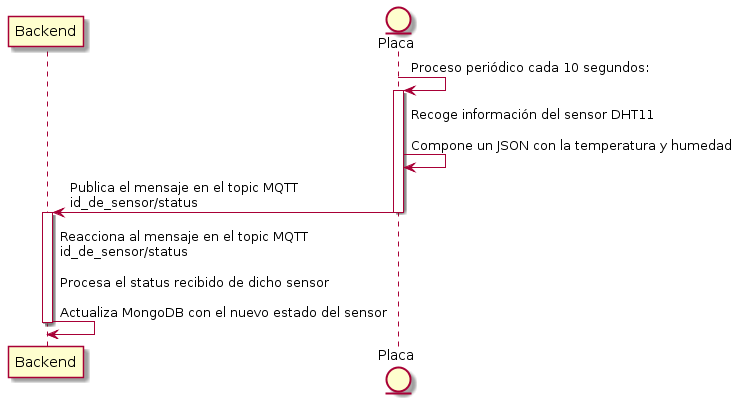
\includegraphics[height=4in]{figures/diagrams/use-cases/sensorInfo.png}
\caption[usecase3sub1]{Diagrama de comunicación entre backend y sensor para comunicar su status\footnotemark}
\label{fig:usecase3sub1}
\end{figure}

\subsection{Fase 1: Lado dispositivo}
\label{ch:Capitulo5.4.1}
El dispositivo se encuentra en un estado permanente de publicación de estado, iterando cada 10 segundos un bucle que recoge la información del sensor de temperatura y humedad, procesando la respuesta en un string con formato \gls{json} con el siguiente contenido \verb|"{\"temperature\": 28, \"humidity\": 53}"| y publicándolo en el topic \textit{thingId/status}. Véase que los contenidos del \gls{json} aquí reflejados son meramente orientativos a la respuesta esperada.

\subsection{Fase 2: Lado servidor}
\label{ch:Capitulo5.4.2}
Precondiciones: el cliente \gls{mqtt} del servidor ha sido inicializado mediante el método \verb|initializeClient| del \verb|mqtt.service.js|, el cual conecta a la dirección \textbf{mqtt://localhost}, y si tiene éxito, mediante el método \verb|_loadSubscriptions| recupera cada thing que haya almacenada en la MongoDB (y que esté vinculada a una habitación) y se suscribe a los topics \verb|answer| y \verb|status| de cada una. Cuando acaba, prepara mediante el método interno \verb|_initMessageListener| una escucha a todos los posibles mensajes \gls{mqtt} que pueda recibir el cliente conectado, y dicha escucha, al recibir un mensaje, lanza el proceso descrito a continuación.

\begin{enumerate}
\item  Se recibe un mensaje \gls{mqtt} con el string \verb|"{\"temperature\": 28, \"humidity\": 53}"| en el topic \textit{thingId/status}. La escucha de mensajes \gls{mqtt} en el \verb|mqtt.service.js| ejecuta un proceso que extrae el id de thing \textit{thingId} y la categoría \textit{status} y llama al método interno \verb|_processMessage|, con esos datos y el string.

\item  Este método delega en \verb|_findSubscriptionIndex| la necesidad de localizar la información de la suscripción correspondiente en la lista interna y, si existe, ejecuta el callback asociado a esta thing para la categoría \textit{status}, en este caso, se trata del método \verb|processStatus| del \verb|sensor.controller.js|.

\item  En el \verb|sensor.controller.js|, se intenta parsear el mensaje mediante el método \verb|_parseMessage|, y se espera que devuelva un objeto JSON.

\item  Si lo devuelve con éxito, actualizará la thing en la MongoDB con el objeto JSON parseado en el campo \verb|sensorMeasures| de la propiedad \verb|typeProperties|, con el método update del modelo \textbf{Thing} (esquema de la MongoDB).
\end{enumerate}

\subsection{Fases paralelas: cálculo de datos generales de la habitación asociada y recuperación de datos en tiempo real}
\label{ch:Capitulo5.4.3}

\begin{figure}[hbt!]
\centering
\label{fig:usecase3sub2}
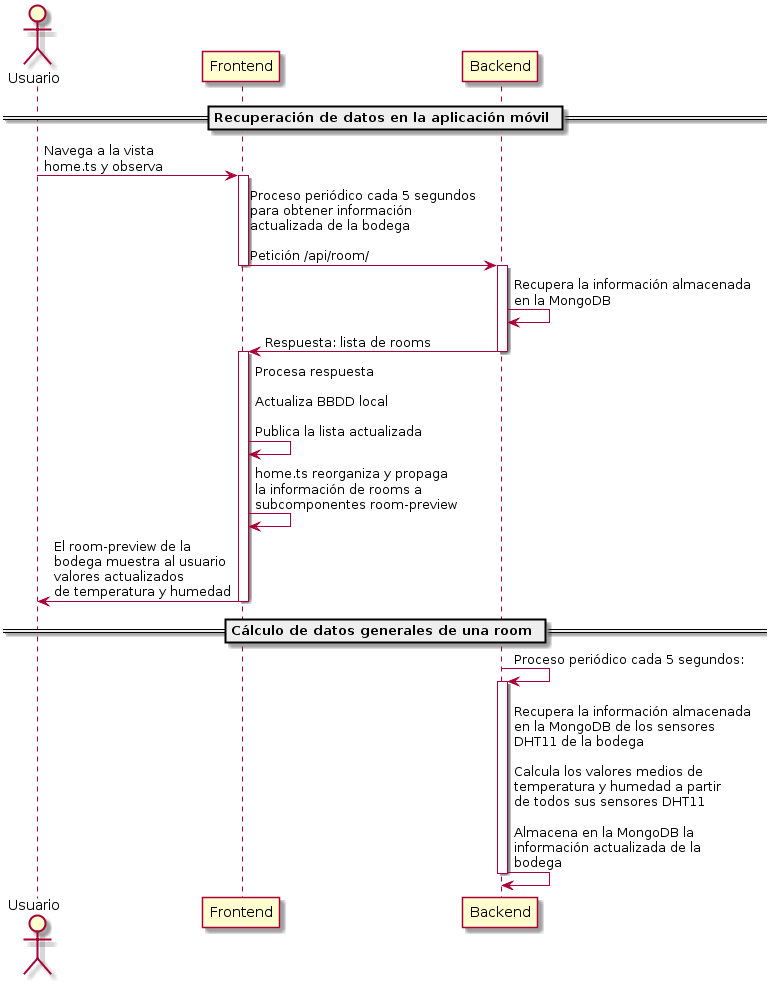
\includegraphics[height=8in]{figures/diagrams/use-cases/sensorInfo2.png}
\caption[usecase3sub2]{Diagrama de procesos en frontend y backend para actualizar información de sensores en una room y mostrarlo al usuario en tiempo real\footnotemark}
\end{figure}

La aplicación backend corre el proceso \verb|roomDaemon| del módulo \verb|room.controller.js| explicado en la sección \ref{makereference4.8.4}, mediante el cual evalúa a intervalos regulares de 5 segundos la información general de una habitación en particular con los cálculos medios de las medidas de los sensores asociados a dicha habitación, y almacena dicha información de la habitación en la colección de Rooms, asociando la información a la habitación.

\vspace{1cm}

De la misma forma y al mismo tiempo, la aplicación frontend corre el proceso \verb|_synchronizeData| de la \verb|room.store.ts| y el proceso \verb|_synchronizeData| de la \verb|thing.store.ts|, mediante los cuales recupera del backend a intervalos regulares de 5 segundos la información actual de rooms y things. Los procesos están descritos en la sección \ref{ch:Capitulo4.7.5}. En pro de la claridad, describiremos el proceso relativo al caso de uso actual hablando únicamente del flujo para las rooms, pero tenga en cuenta el lector que a la vez ocurre el proceso paralelo para las things, con sus métodos homónimos en sus respectivos módulos homónimos.

\begin{enumerate}
\item La lógica asociada a la vista que esté usando el usuario en ese momento es la que se suscribe al observable \verb|roomsChange| de la \verb|room.store.ts|, siguiendo el patrón Observer/Subscribe. Puede darse el caso tanto en la vista global \verb|home.ts|, en la que observamos los datos resumidos de todas las habitaciones registradas y será la descrita en esta subsección, como en la vista particular de la room \verb|room.ts|, para el caso actual la bodega, en la que observaremos los datos generales de la habitación así como los datos individuales de cada dispositivo asociado.
\item Según se ha descrito al principio de esta subsección, cuando la aplicación recupera los datos y progresa la ejecución del método \verb|_synchronizeData| de la \verb|room.store.ts|, se notifica al suscriptor del paso anterior la lista actualizada de rooms, de forma que se ejecuta el desencadenante del suscriptor creado en el constructor de \verb|home.ts|. Dicho desencadenante lanza el método privado \verb|indexThingsInRooms| para encajar la información actualizada de cada thing en cada room asociada, dentro de una lista de rooms.
\item Mediante el paradigma de componentes, el template \verb|home.html| instancia un componente \verb|room.preview.component| por cada room de la lista anterior, y le transfiere la información de dicha room. El template de dicho componente encuentra los valores generales de temperatura y humedad dentro del campo \verb|sensorMeasures| del objeto \verb|room| y los muestra finalmente como valores numéricos para información del usuario.
\end{enumerate}